This section will be focused on analysing any problems the group may face, how to approach them, and how they should be handled.

\section{Problem statement}

The problem presented to the group is how to make a robot move from point A to point B, with the help of different sensors, including ultrasound and infrared, and to make use of autonomous algorithms to avoid obstacles. \\

Problem statement:
\begin{enumerate}
\item[•]The robot should be able to move from A to B
\item[•]It should be able to stop at a predetermined point
\item[•]It needs to manoeuvre around obstacles
\end{enumerate}

\section{Problem analysis}
\subsection{Mobility from A to B}
The robot receives a coordinate to reach, and will use its own starting point to determine a direction to drive towards the given coordinate. The robot will need a way to control its movement and direct current to function optimal.\\
The robot needs a way to effectively regulate speed and also steer itself autonomously. To dictate how quickly the robot moves, the robot will need some system that allows it to move around on a flat surface, the robot needs to be able to move around from point A to point B.
.\

\subsection{Predetermined end point}
After starting, the robot needs to know when to stop. The pre-determined end-point could consist of a series of circles which the robot needs to detect, or just be coordinates in a theoretical coordinate system.

\subsection{Obstacle avoidance}
As part of its functionality, the robot needs to be able to see objects that are in front of it and avoid them. After avoiding an obstacle, the robot needs to determine where it is compared to the goal, and go towards that again.

\section{Behaviour}
The robot is expected to fulfil the previously mentioned tasks on it's own. To do this, a few algorithms are to be utilized. This section will describe some of the ideas and considerations made by the group.\\\\
To solve the problem of going from A to B, 2 methods have been considered. Both of these assume that both the start and end point are known. The first and simplest method is simply to manually turn the robot towards the goal, and letting the robot drive until it detects the goal. The other, and chosen, method is to know the coordinates for the end compared to where the robot starts.\\\\
This method also solves the second problem by reading the tach count from the motors, and calculating the distance driven from these. The other method of finding the end point is by using a few sensors in a line sensing fashion, giving the robot some space to work with if the calculations are not perfect.\\\\
The last problem, obstacle avoidance, only one viable solution was discussed in the group: using 3 ultrasound sensors to detect obstacles around the robot. The placement of these, however, was considered. Due to previous experience with object avoidance, it was chosen to mount 1 sensor in the middle looking forward, and 1 to either side of this, turned 90 degrees(See figure \ref{Hardware_diagram}). This was chosen over having the side sensors turned 45 degrees because tests in the previous project showed ultrasound sensors to give inconsistent results when reading data from obtuse angles.

\begin{figure}[!ht]
	\centering
	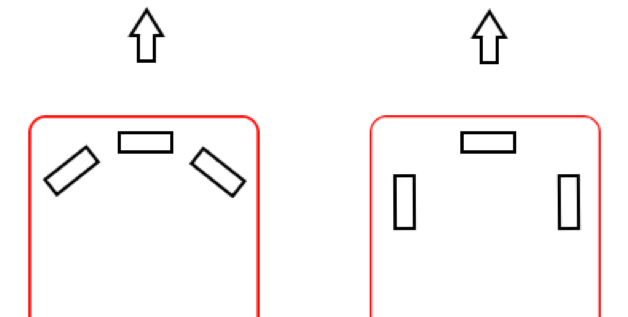
\includegraphics[width=0.7\textwidth]{figures/sensorMountingTheory.PNG}
	\caption{\text{Proposed placement of sensors, right shows the chosen placement}}
	\label{Hardware_diagram}
\end{figure}